\chapter{El LHC y el detector ATLAS}
% \addcontentsline{toc}{chapter}{El LHC y el detector ATLAS}
\chaptermark{El LHC y el detector ATLAS}


El Gran Colisionador de Hadrones (\textit{\textbf{L}arge \textbf{H}adron \textbf{C}oliider} (LHC)) \cite{Evans:1129806} es el acelerador de hadrones del Centro Europeo para la Investigación Nuclear (CERN), ubicado en la frontera entre Francia y Suiza. Posee una longitud de 27 km y fue construido en el mismo túnel en el que funcionaba el acelerador $e^{+}e^{-}$ LEP (etre 1989 y 2000), a una profundidad variable entre $50$ y $174$ m de la superficie.

El LHC está diseñado para colisionar protones (e iones pesados) a una energía de centro de masa de $\sqrt{s}=14$ TeV. Para ello el CERN posee un complejo de aceleradores que, en sucesivas etapas, incrementan la energía de los protones (Figura \ref{acc_complex}). El último de los aceleradoes es el LHC, donde los protones circulan en direcciones opuestas por cavidades de ultra alto vacío a una presion de $10^{-10}$ torr. El mismo cuenta con $1232$ dipolos magnéticos superconductores enfriados a $1.9$ K, que generan un campo magnético de $8.4$ T, lo que permite acelerar a los protones y mantenerlos en su órbita circular. El sistema de focalización de los haces consiste de $392$ cuadrupolos magnéticos que generan campos magnéticos de $6.8$ T.

\begin{figure}[ht]
\centering
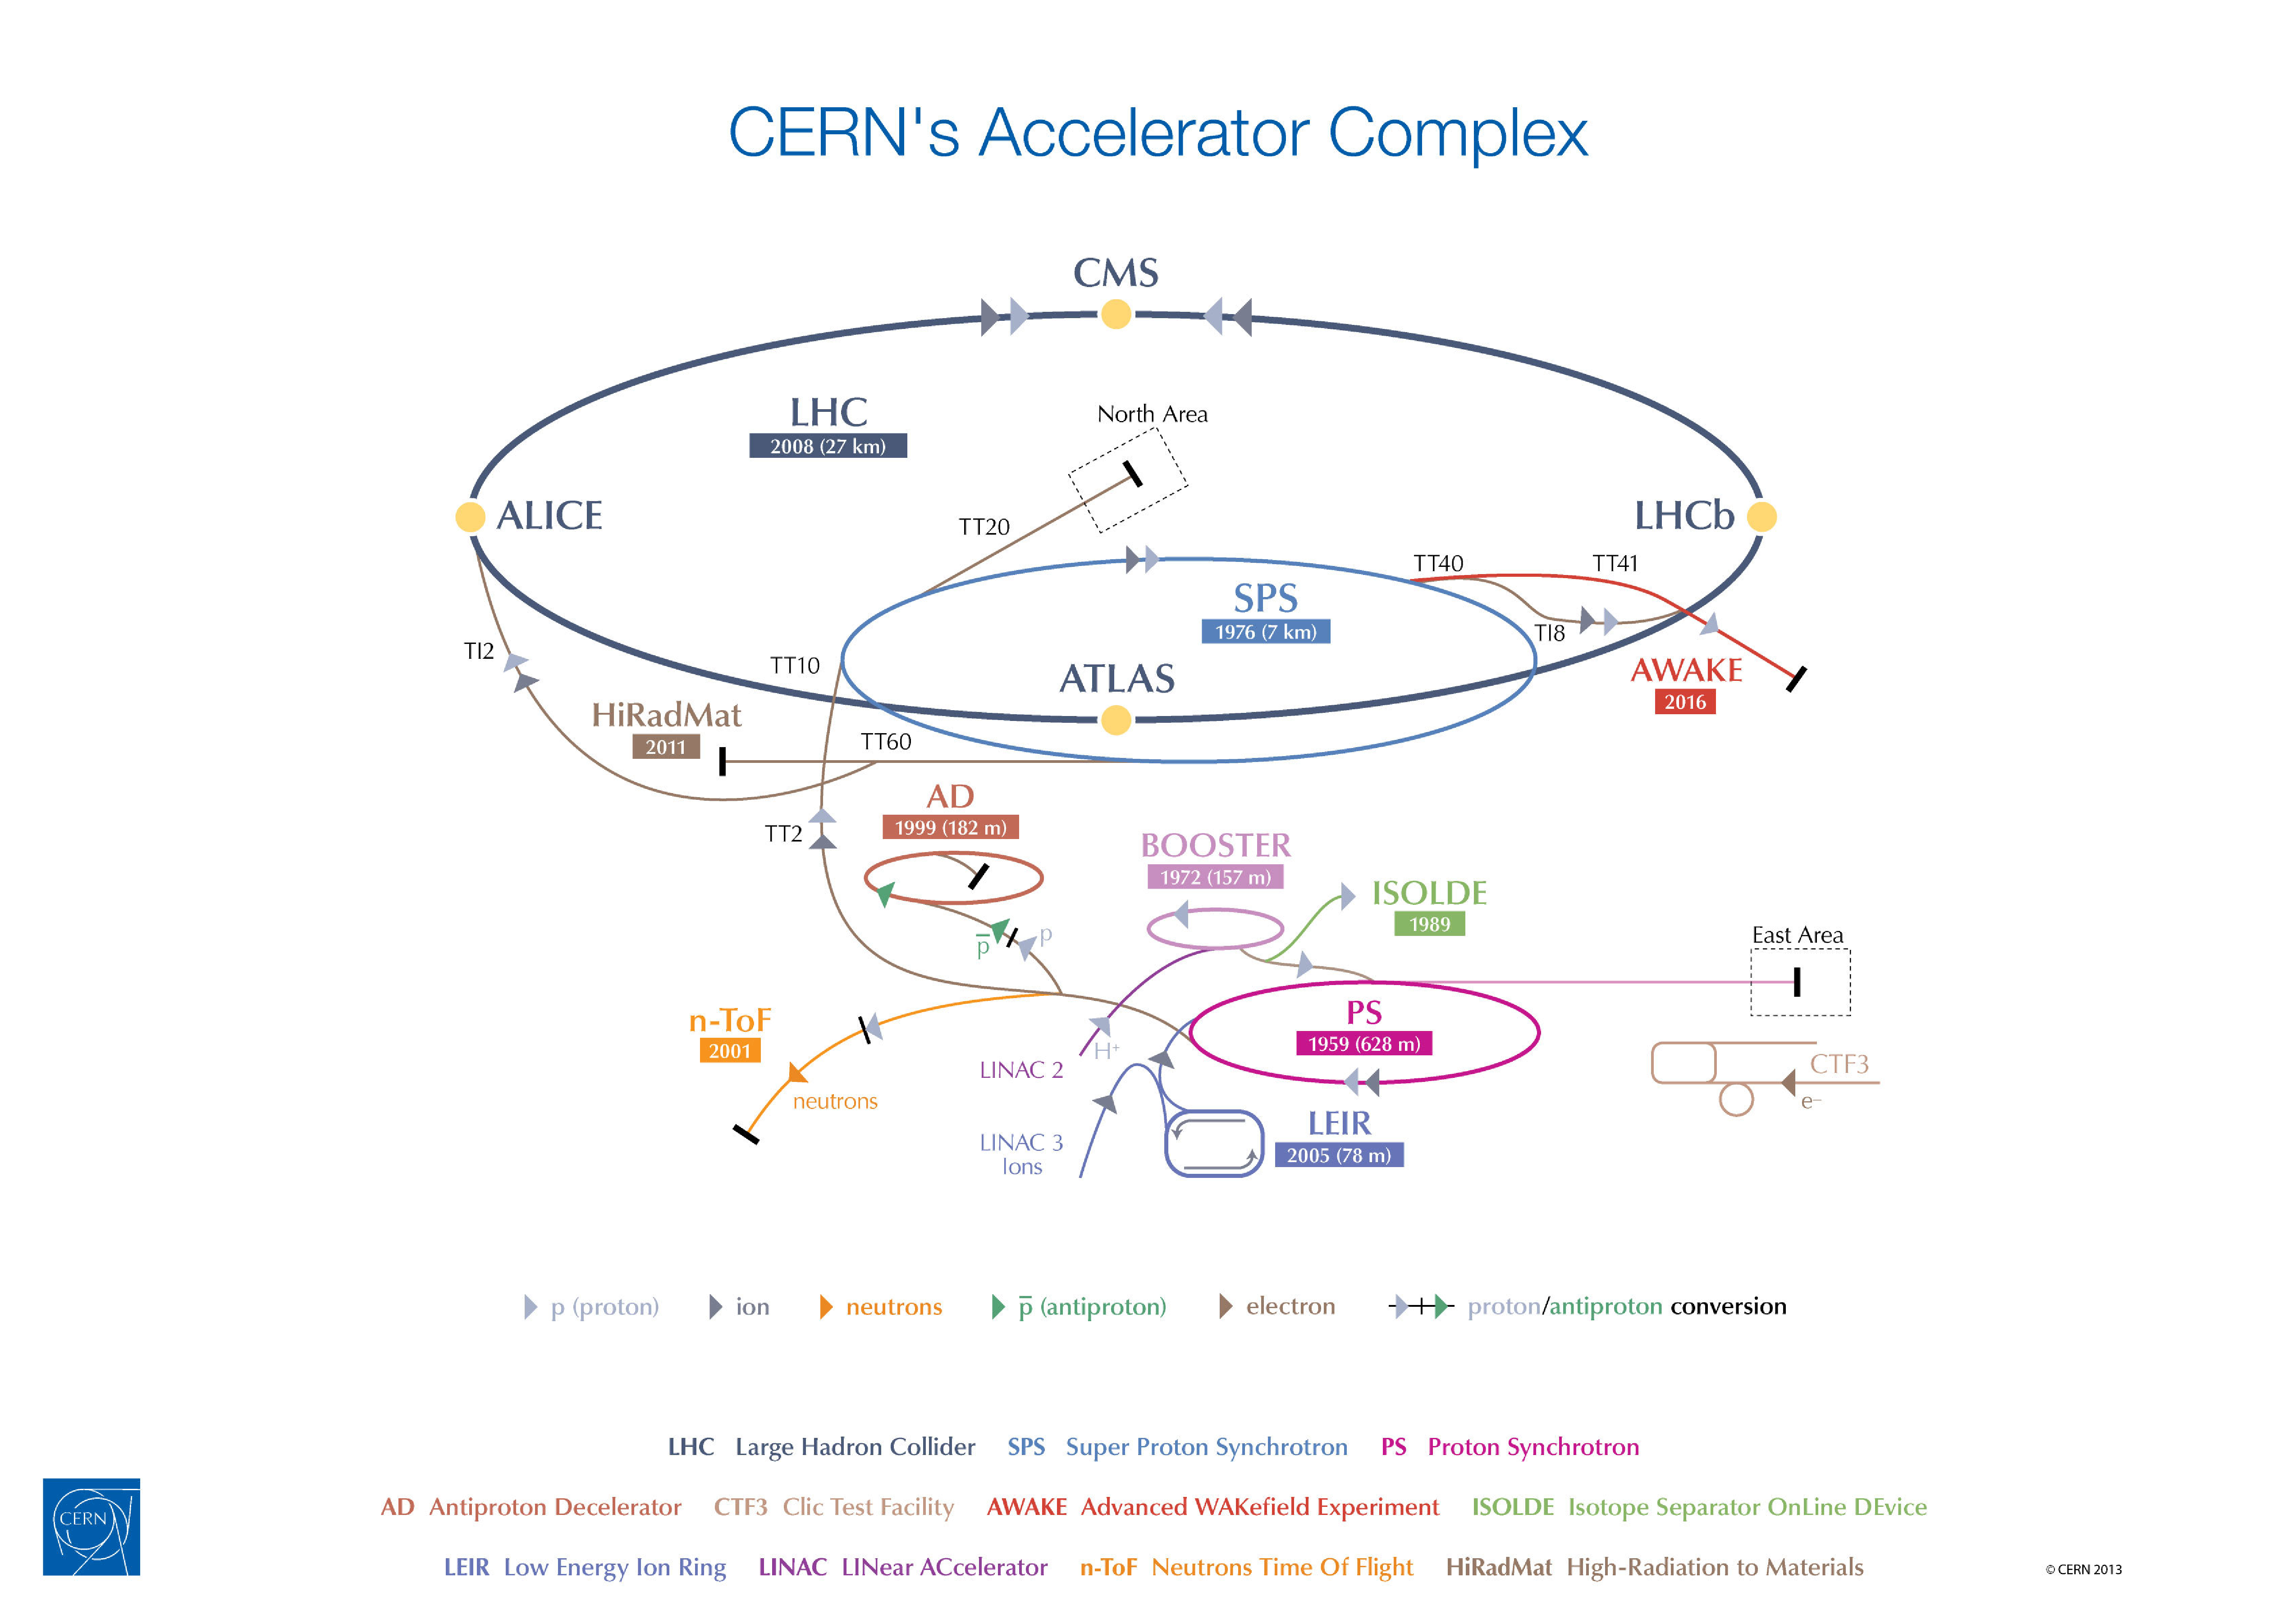
\includegraphics[width=1\textwidth]{acc_complex.eps}
\caption{EComplejo de aceleradores del CERN, incluyendo al LHC y a la serie de aceleradores utilizados para proveer de protones al LHC. También pueden verse los diferentes experimentos ubicados en el acelerador.}
% \vspace{0.2cm}\footnotesize\textbf \sl{...}\vspace{0.2cm}
\label{acc_complex}
\end{figure}

El diseño del LHC contempla trenes de $2808$ paquetes de $\sim 10^{11}$ protones cada uno, espaciados temporalmente en $25$ ns. Para caracterizar el funcionamiento del acelerador, se utiliza una varaible denominada luminosidad instantánea. Se define como el número de partículas por unidad de tiempo y unidad de área:

\begin{equation}
\mathcal{L}=f_{rev}n_{b}\frac{N_{1}N_{2}}{A}
\end{equation}

donde $f_{rev}$ es la frecuencia de revolución ($\sim$ 11 kHz), $n_{b}$ es el número de \textit{bunches} (paquetes de protones) por haz, $N_{i}$ es el número de partículas en cada \textit{bunch} y \textit{A} es la sección efectiva del haz, que puede expresarse en término de los parámetros del acelerador como:

\begin{equation}
A=\frac{4 \pi \epsilon_{n}\beta^{*}}{\gamma F}
\end{equation}

donde $\epsilon_{n}$ es la emitancia transversal normalizada (la dispersión transversal media de las partículas del  haz en el espacio de coordenadas e impulsos), $\beta^{*}$ es la función de amplitud en el punto de interacción, relacionada al poder de focalización de los cuadrupolos), $\gamma$ es el factor relativista de Lorentz y \textit{F} es un factor de reducción geométrico, debido al ángulo de cruce de los haces en el punto de interacción.

... Datos actuales

\section{El detector ATLAS}

ATLAS (\textit{\textbf{A} \textbf{T}oroidal \textbf{L}HC \textbf{A}paratu\textbf{S}})  \cite{PERF-2007-01} es uno de los experimentoas multipropósito del LHC, diseñado para estudiar las colisiones protón-protón a altas energías provistas por el LHC.

El esquema del detector se puede observar en la figura \ref{ATLAS}. Tiene una smietría aproximadamente cilíndrica, y está compuesto de distintos subdetectores que cumplen diversas funciones (ver Figura \ref{cross_section_2}). En la zona más próxima al haz se encuentra el detector interno de trazas (ID), compuesto de un detector de píxeles, un detector de bandas de silicio (SCT) y un detector de radiación de transición (TRT). Envolviendo el ID se encuentra un solenoide superconductor que genera un campo magnético de $2$ T, el cual curva la trayectoria de las partículas cargadas para así medir su impulso.

\begin{figure}
\centering
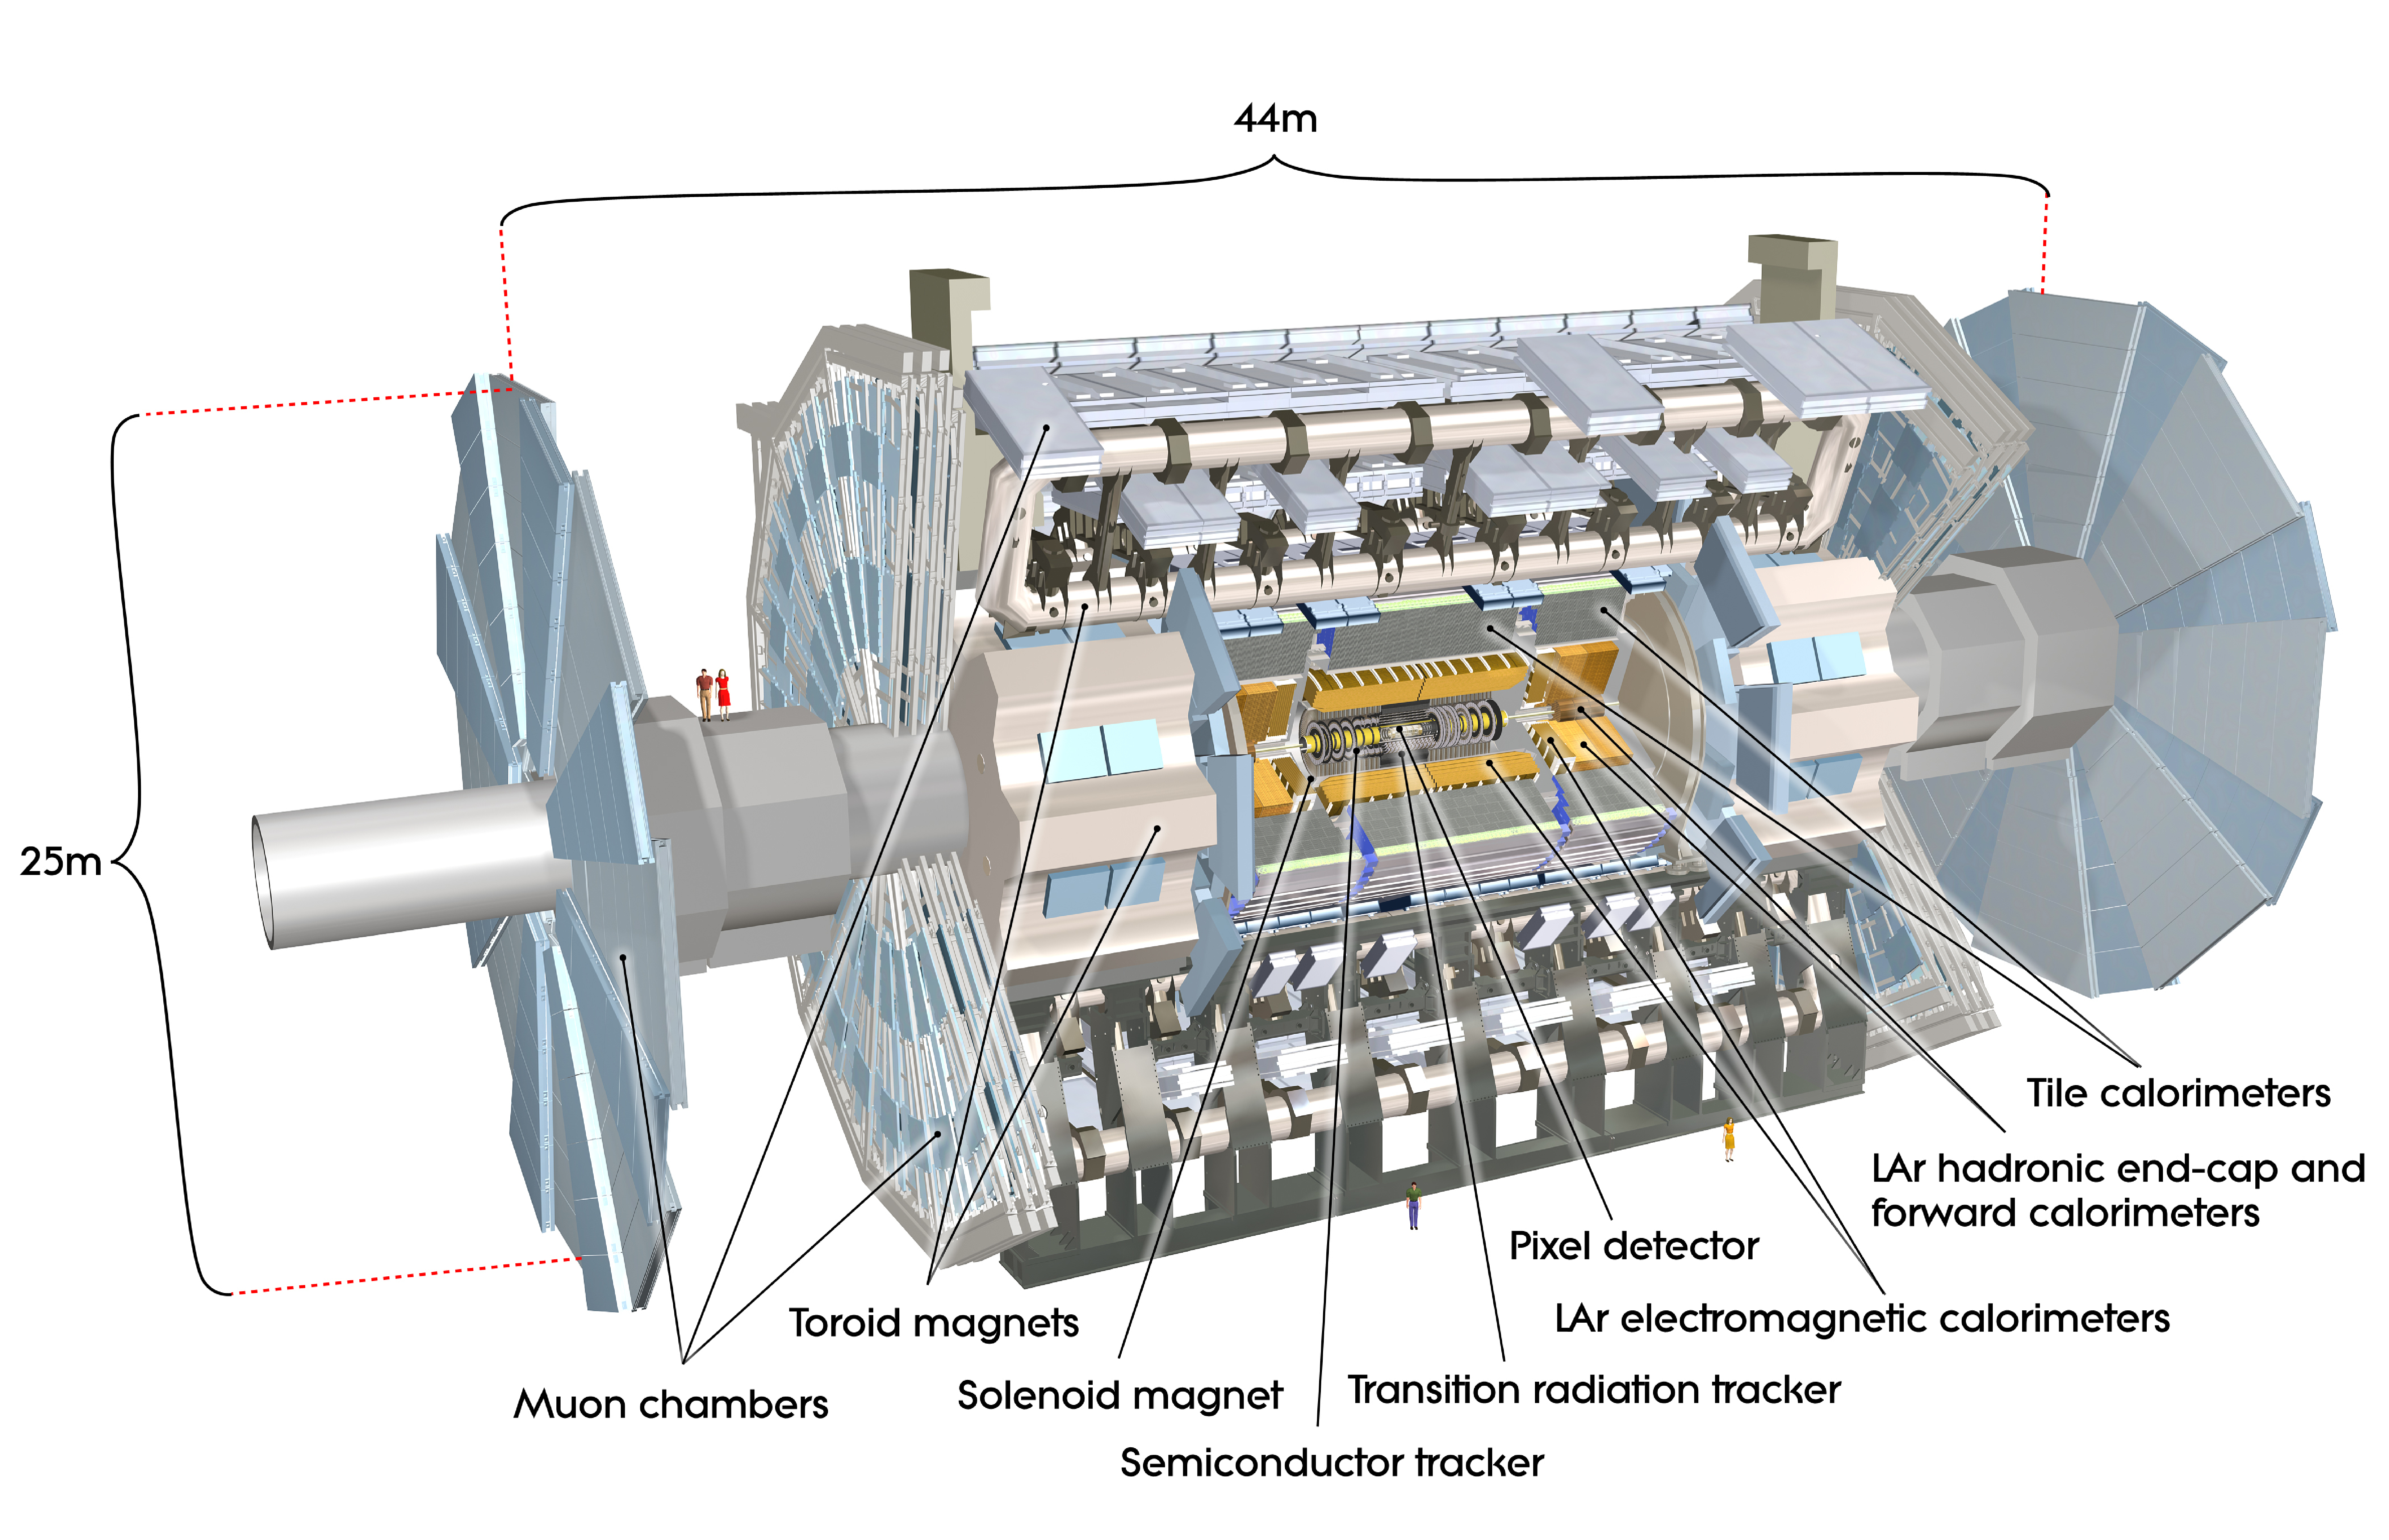
\includegraphics[width=1\textwidth]{ATLAS.eps}
\caption{Esquema general del detector de ATLAS.}
% \vspace{0.2cm}\footnotesize\textbf \sl{...}\vspace{0.2cm}
\label{ATLAS}
\end{figure}

\begin{figure}
\centering

\includegraphics[width=0.7\textwidth]{cross_section_2.eps}
\caption{Esquema del corte transversal del detector de ATLAS, ilustrando los distintos subdetectores y el pasaje de las distintas partículas.}
% \vspace{0.2cm}\footnotesize\textbf \sl{...}\vspace{0.2cm}
\label{cross_section_2}
\end{figure}

A continuación se ubica el sistema de calorímetros: el calorímetro electromagnético (ECAL) que mide la energía depositada por fotones y electrones, y el calorímetro hadrónico (HCAL) para medir la energía de los jets y hadrones.

Finalmente, se encuetra el espectrómetro de muones (MS) intercalado con un sistema de imanes toroidales, que generan un campo magnetico necesario apra curvar la trayectoria de los muones dentro del detector.

El detector ATLAS se divide geométricamente en dos regiónes, la parte central denominada \textit{barrel} y la región extrema \textit{endcap}. En la región \textit{barrel} los detectores se ubican en forma de cilindros concentricos alrededor del eje del haz, mientras en en la región \textit{endcap} se disponen como discos perpendiculares a la direccion del haz. 

\section{Sistema de coordenadas}

El sistema de coordenadas de ATLAS corresponde a un sistema cartesiano, cuyo origen coincide con el punto de interacción nominal. El eje \textit{z} corresponde al eje del haz, el eje \textit{x} se define desde el punto de interacción hacia el centro del LHC, y el eje \textit{y} se define apuntando hacia arriba.

Es conveniente además definir un sistema de coordenadas cilíndricas. Donde el radio \textit{R} representa la distancia perpendicular al haz. El ángulo azimutal $\phi$ es medido alrededor del eje del haz, y el ángulo $\theta$ se mide con respecto al eje del haz. 

Una cantidad muy importante utilizada en física de altas energías es la llamada rapidez:

\begin{equation}
w=\frac{1}{2}\ln\left( \frac{E+p_{z}}{E-p_{z}}\right)
\end{equation}

donde \textit{E} es la energía total de la partícula y $p_{z}$ es la componente longitudinal de su impulso. En el límite de altas energías esta cantidad se aproxima (en forma exacta para objetos no masivos) por la llamada pseudorapidez, $\eta$, relacionada con el ángulo polar $\theta$ como:

\begin{equation}
\eta =-\ln \tan\left( \frac{\theta}{2} \right)
\end{equation}

La razón detrás de esta transformación de coordenadas es el hecho que la multiplicidad de partículas producidas es aproximadamente constante como función de $\eta$, y que la diferencia de pseudorapidez entre dos partículas es invariante frente a transformaciones de Lorentz a lo largo de la dirección del haz. En el caso de colisiones hadrónicas, la fracción del impulso del protón adquirida por cada uno de las partones interactuantes es desconocida. Parte de este impulso es transferido en la interacción dura, mientras cierta fracción remanente escapa el detector a lo largo del haz. Así, no es posible reconstruir el movimiento longitudinal del centro de masa en la interacción, y aplicar leyes de conservación sobre la cinemática de cada evento. Sin embargo, dado que los protones inciden a lo largo de la dirección del haz, el impulso total transverso es conservado durante la colisión. Por esta razón, solo las componentes transversales son utilizadas en la descripción de la cinemática del evento, por ejemplo $p_{T}$ ($=p\sin\theta$). En términos de la pseudorapidez, se define la energía transversa ($E_{T}=E\sin\theta$) de una partícula como:

\begin{equation}
E_{T}=\frac{E}{\cosh \eta}
\end{equation}

donde \textit{E} es su energía total.

\section{Los subdetectores de ATLAS}

\subsection{El detector interno}

\begin{figure}
\centering
\includegraphics[width=0.70\textwidth]{ID.eps}
\caption{Esquema general del detector de ATLAS.}
% \vspace{0.2cm}\footnotesize\textbf \sl{...}\vspace{0.2cm}
\label{ID}
\end{figure}

El detector interno es el más próximo al haz y esta contenido dentro de un solenoide que provee un campo magnetico de $2$ T. Un esquema general del mismo se puede observar en la figura \ref{ID}. Está compuesto por distintos detectores como muestra la figura \ref{ID_2}.

\begin{figure}
\centering
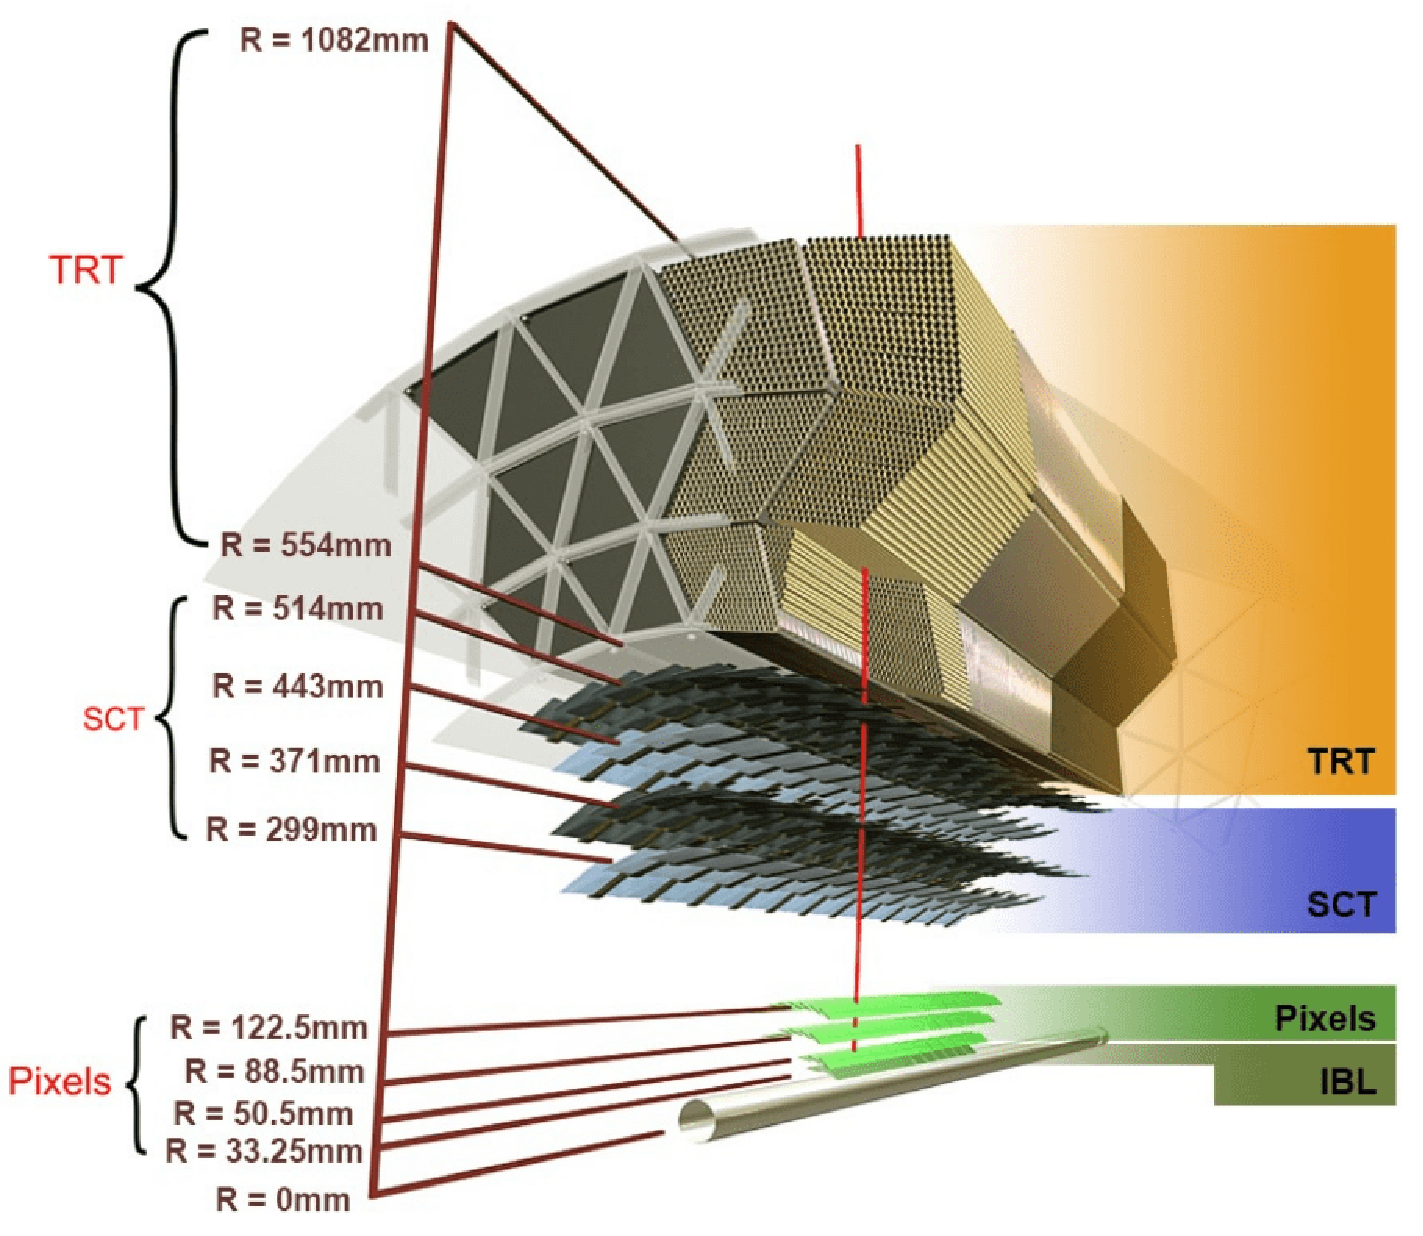
\includegraphics[width=0.60\textwidth]{ID_2.eps}
\caption{Esquema del detector interno mostrando la traza de una partícula cargada de $p_{T}=10\egev$ atravesándolo. La trayectoria atraviesa el tubo del haz de  erilio, las tres capas del detector de píxeles de silicio (Pixels), las cuatro capas dobles de sensores semiconductores (SCT), y aproximadamente 36 tubos contenidos en los módulos del detector por radiación de transición (TRT).}
% \vspace{0.2cm}\footnotesize\textbf \sl{...}\vspace{0.2cm}
\label{ID_2}
\end{figure}

\vspace{0.5cm}

{\bf Detector de píxeles }

Es el más interno de los detectores, construído para medir la posición de las trazas de partículas cargadas con la más alta precisión posbile y es de vital importancia para la reconstrucción de los vértices primarios y secundarios. En la región \textit{barrel} consiste en tres cilindros, mientras que la \textit{endcap} tres discos. El principio de detección para partículas cargadas es la medida de la deposición de la carga inducida en una capa de silicio por ionización. El sistema contiene un total de $80.4$ millones de sensores, cada uno con una resolucion intrínseca de entre $12$ $\mu$m y $110$ $\mu$m. AGREGAR IBL.

\vspace{0.5cm}

{\bf Detector Semiconductor de Trazas (SCT) }

Se encuentra por fuera del detector de píxeles y está deseñado para medir las trazas con alta precisión en la zona intermedia del detector. A diferencia del detector de píxeles, estos sensores de silicio están segmentados en micro bandas, dada la mas baja multiplicidad de partículas. La resolución varía entre $16$ $\mu$m y $580$ $\mu$m. En la región \textit{barrel} los módulos de SCT estan dispuestos en 4 capas concéntricas, mientras que en la región \textit{endcap} consiste en 9 discos transversales al eje del haz.

\vspace{0.5cm}

{\bf Detector de Radiación de Transición (TRT) }

Es el detector más externo del ID y está diseñado, no solo para detectar partículas cargadas, sino también para detectar la radiación de transición que permite distinguir entre partículas cargadas pesadas y livianas (diferenciar entre $\pi^{\pm}$ y $e^{\pm}$ por ejemplo). El TRT se basa en el uso de tubos detectores que pueden operar a alta frecuencia de eventos gracias a su pequeño diámetro ($4$ mm) y el aislamiento de sus hilos centrales en volúmenes de gas individuales. La región barrel contiene $50000$ tubos paralelos al eje del haz y la región endacap $420000$ tubos orientados radialmente. Su resolucion es de $0.17$ mm. EXPLICAR POR QUE RADIACION.

\subsection{Calorímetros}

El sistema de calorímetros de ATLAS está sdiseñado para medir la energía y la posición de las partículas, mediante la absorción de la energía depositada por las cascadas de partículas secundarias que estas generan en el material del mismo. Además, permite discriminar electrones y fotones de jets, medir el desbalance de energía transversa y la selección online de eventos potencialmenteinteresantes (\textit{trigger}). Este sistema incluye un calorímetro electromagnético (ECAL) y otro hadrónico (HCAL), como muestra la figura \ref{Cal}.

\begin{figure}
\centering
\includegraphics[width=0.70\textwidth]{Cal.eps}
\caption{Sistema de calorímetros del detector ATLAS.}
% \vspace{0.2cm}\footnotesize\textbf \sl{...}\vspace{0.2cm}
\label{Cal}
\end{figure}

{\bf Calorímetro electromagnético }

En la figura \ref{ecal} se puede ver el esquema del mismo. La región \textit{barrel} de este sistema consiste en un calorímetros de muestreo que utiliza plomo como material absorbente. Las partículas incidentes iteractúan con este material, creando una lluvia de partículas cargadas y neutras. Las partículas cargadas ionizan el medio activo (LAr) colocado entra las placas de plomo, donde los electrones liberados son colectados en un electrodo central de kaptón/Cu hacia donde derivan por acción del campo eléctrico aplicado. La señal total en el medio activo es así poroporcional a la energía total real de la partícula incidente.

\begin{figure}
\centering
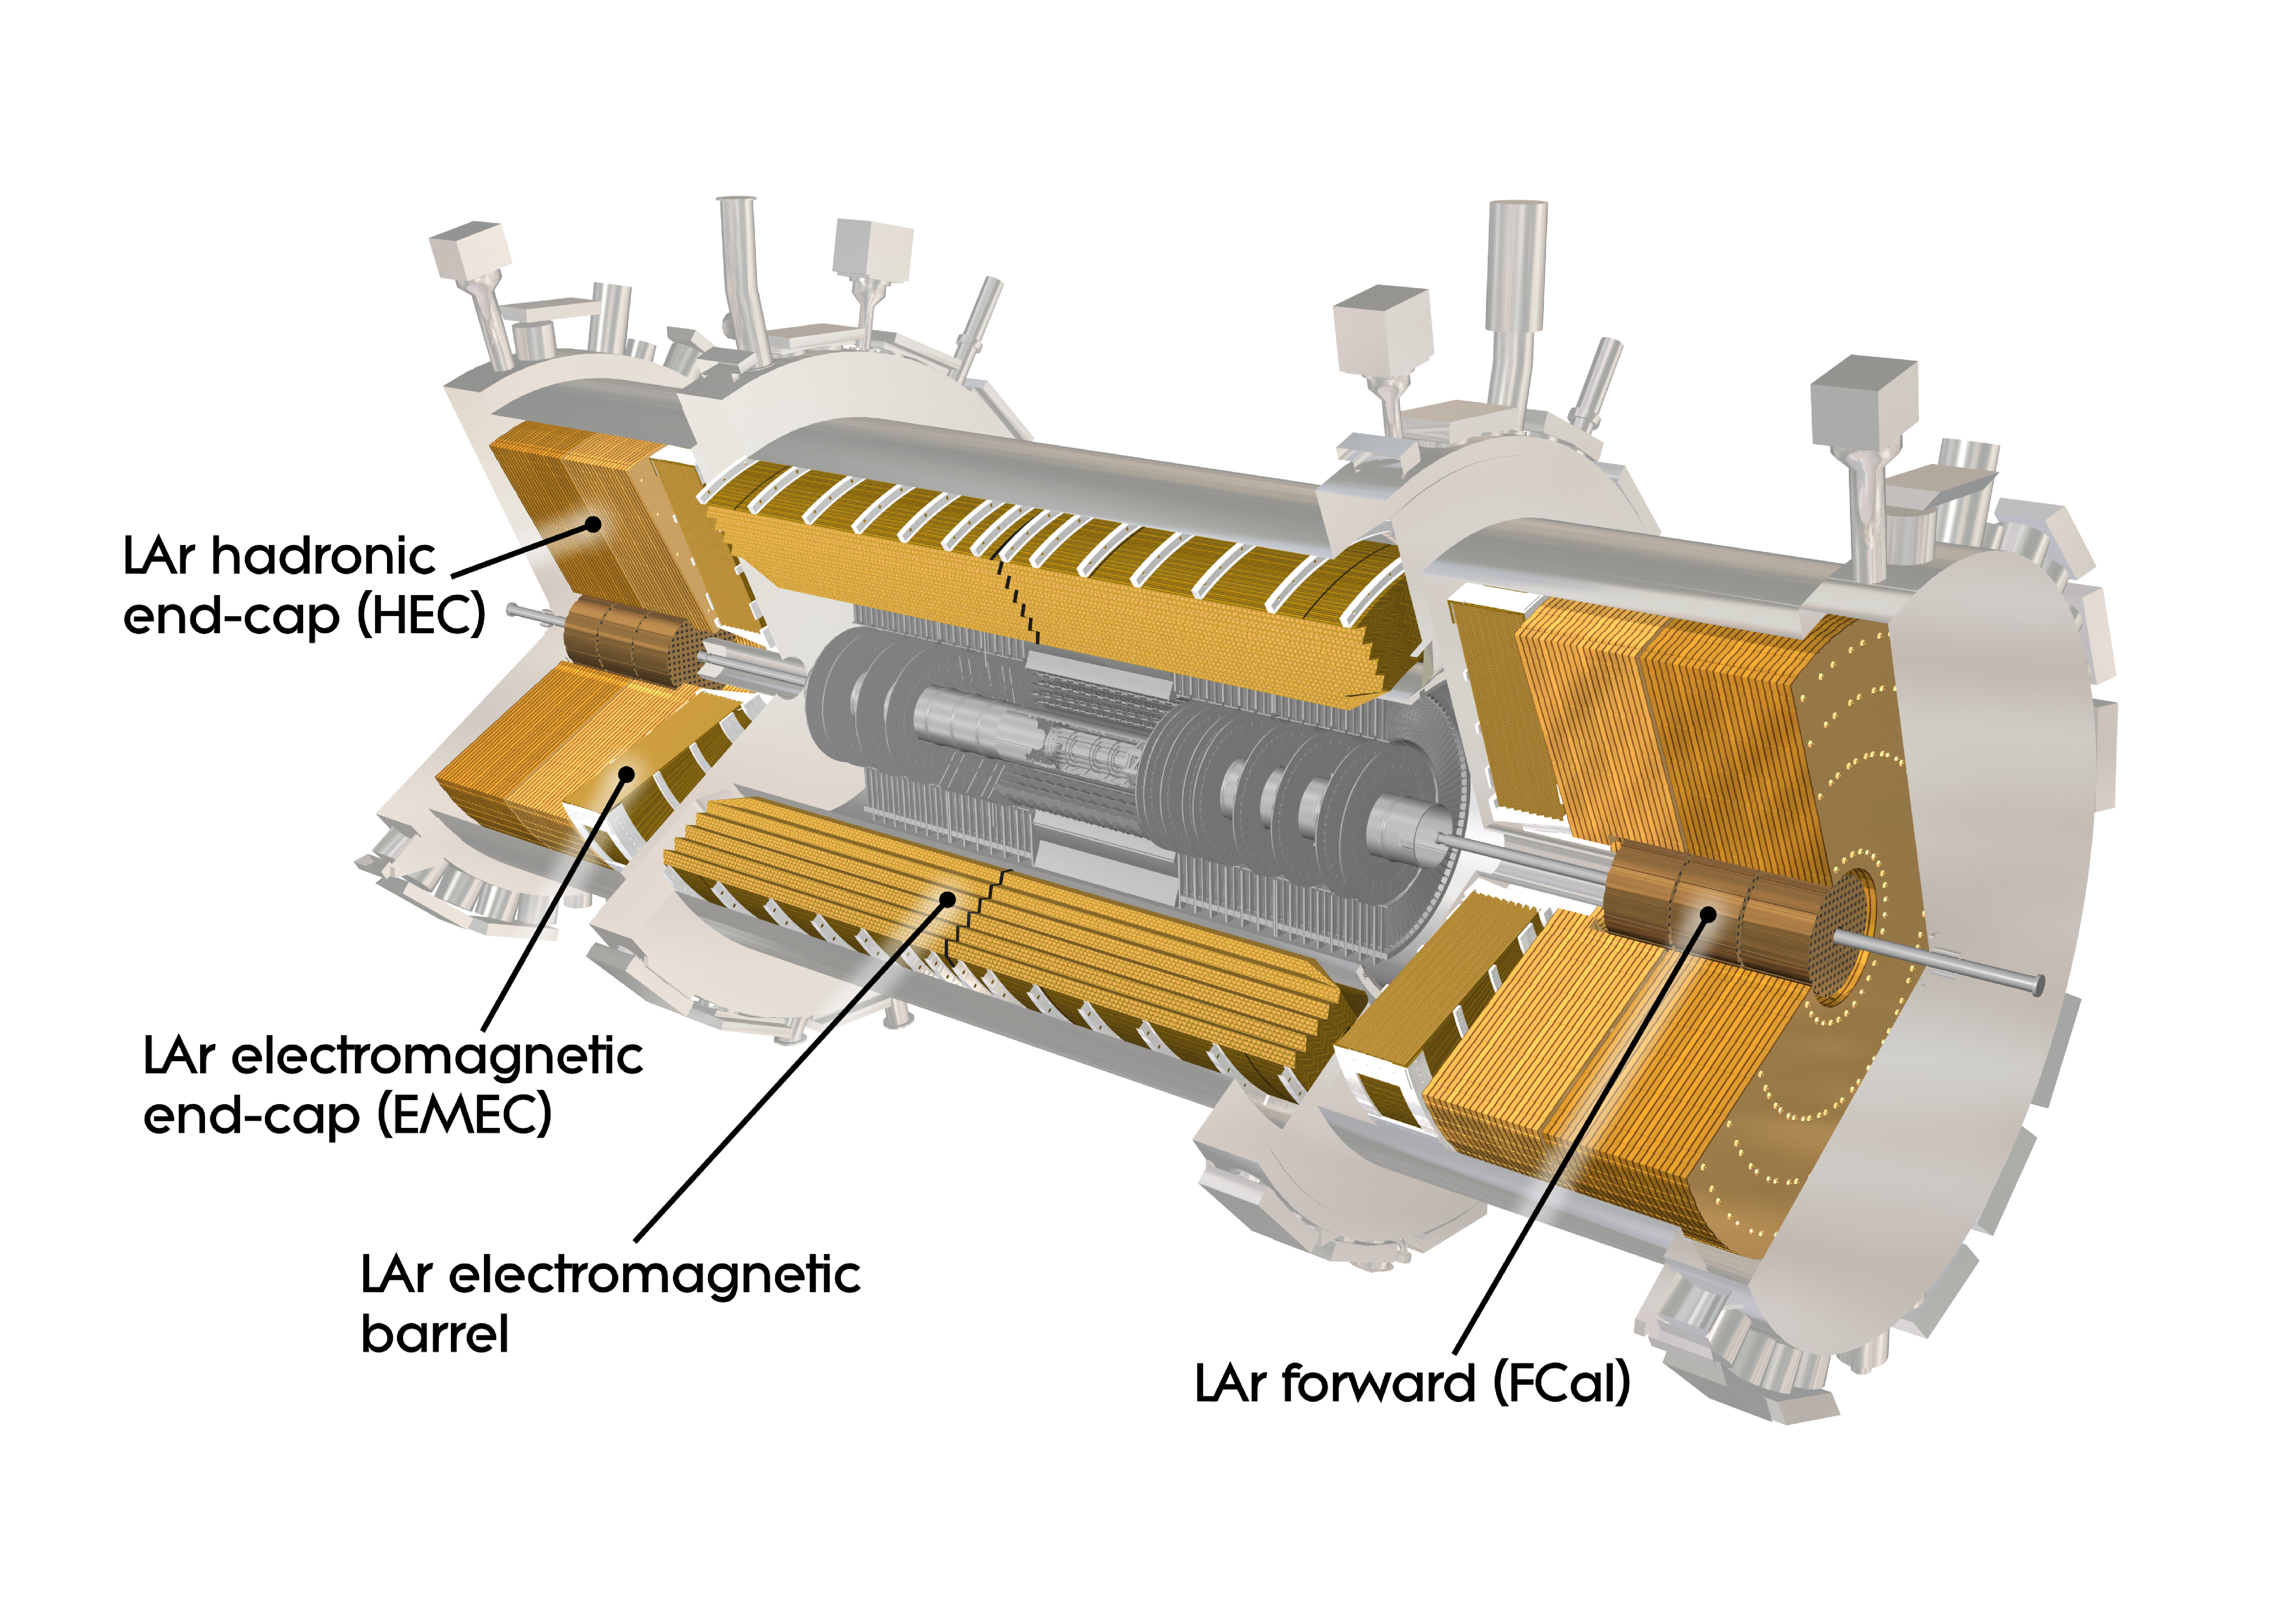
\includegraphics[width=0.70\textwidth]{ecal.eps}
\caption{ECAL del detector ATLAS.}
% \vspace{0.2cm}\footnotesize\textbf \sl{...}\vspace{0.2cm}
\label{ecal}
\end{figure}

El ECAL se divide en una parte central y los \textit{endcaps}. En la región de transición entre el \textit{barrel} y el \textit{endcap} se encuetra una zona no isntrumentada, por donde se conecta el detector. Esta región denominada \textit{crack}, está comprendida entre $1.37 < |\eta| < 1.52$. Es por este motivo que la mayoría de los análisis se requiere que los candidaos a fotones/electrones estén fuera de la región \textit{crack}.

{\bf Calorímetro hadrónico }

El calorímetro hadrónico cubre el rango $|\eta|< 4.9$ usando diferentes materiales. La parte del \textit{barrel} de este sistema utiliza acero como absorbente y tejas centelladoras como material activo. Las tejas están ubicadas radialmente y apiladas en profundidad. En la región de \textit{endcaps}, el calorímetro hadrónico se compone de dos ruedas perpendiculares al tubo del haz, hechas con placas de cobre y tungsteno como material absorbente y argón líquido como material activo. Estos detectores extienden la aceptancia del calorímetro de ATLAS hasta cubrir prácticamente la totalidad de ángulo sólido del punto de colisión.

\subsection{Espectrómetro de muones}

Los muones de alto $p_{T}$ generados en el punto de interacción tienen un altísimo poder de penetración y son poco interactuantes. Por ello el espectrómetro de muones se encuentra situado en la parte más exterior del detector ATLAS, alrededor del sistema de imanes de toroides, y está diseñado para obtener mediciones de alta precisión de posición e impulso de muones de alto $p_{T}$ . Este es el subdetector más grande y el que le da a ATLAS su tamaño característico (ver figura \ref{muon}. 

\begin{figure}
\centering
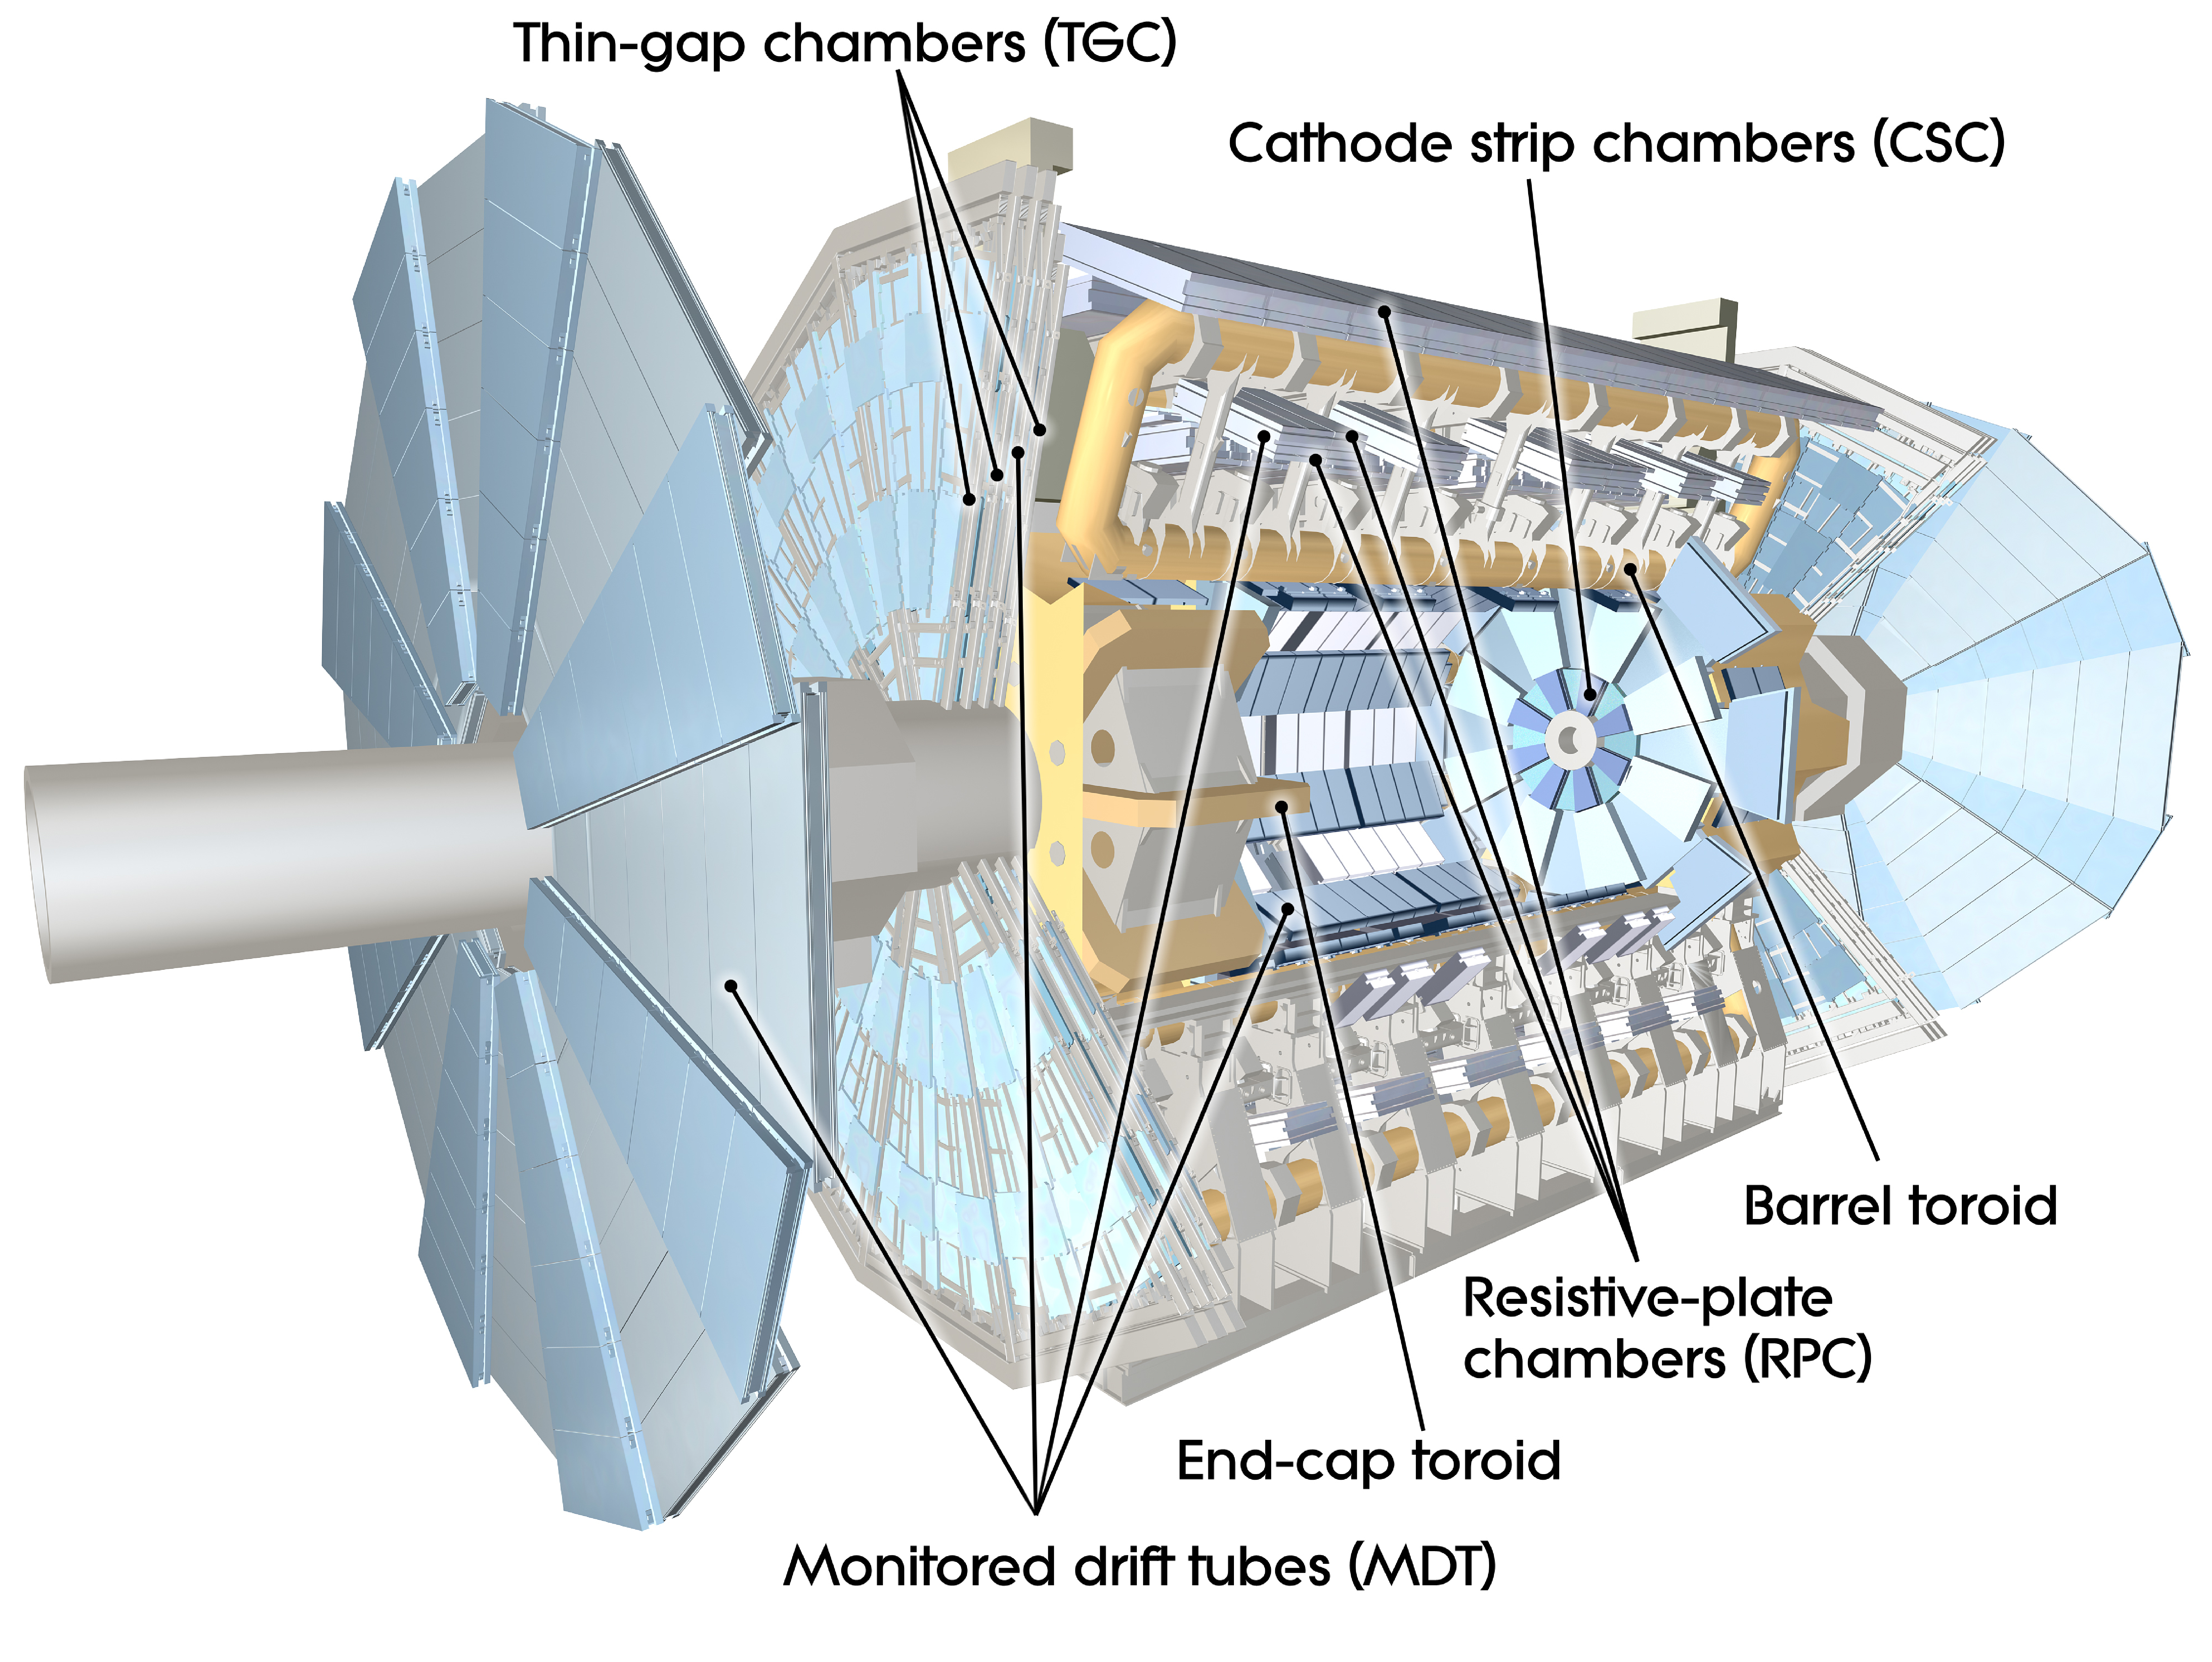
\includegraphics[width=0.60\textwidth]{muon.eps}
\caption{Espectrómetro de muones del detector ATLAS.}
% \vspace{0.2cm}\footnotesize\textbf \sl{...}\vspace{0.2cm}
\label{muon}
\end{figure}

Los muones al ser altamente penetrantes, son las únicas partículas (excepto las invisibles que no interactúan) que llegan al sistema de muones. Estos pierden parte de su energía mientras penetran las capas internas de ATLAS antes de llegar al espectrómetro de muones. La pérdida de energía es tenida en cuenta utilizando los depósitos de energía en los distintos calorímetros.

\section{Sistema de \textit{trigger}}

El diseño del LHC permite tener una frecuencia de cruces de haces de 40 MHz y alrededor de 23 interacciones por cruce, lo que da una tasa de interacción protón-protón del orden del GHz. Debido a que el almacenamiento y el poder de cómputo de los datos recolectados son limitados, y considerando que no todos los eventos son de interés, es necesario reducir el flujo de datos incidentes a una frecuencia de $\sim 400$ Hz \cite{PERF-2011-02}. El sistema de trigger, es el encargado de filtrar los eventos que son de interés, para su poseterior análisis. 

El sistema de trigger de ATLAS consiste en una selección de eventos basada en tres niveles: Level 1 (L1), Level 2 (L2) y el Event Filter (EF), siendo los dos últimos los que coforman el High Level Trigger (HLT). Cada nivel permite analizar los eventos con mayor detalle, aumentando la precisión de los criterios de selección y la complejidad de los algoritmos utilizados.

El primer nivel de trigger se encarga de la selección inicial, reduciendo la frecuencia de eventos que pasan al siguiente nivel a $\sim 75$ kHz. Debido al tamaño limitado de las memorias temporales donde se guardan los datos de cada subdetector y al considerable tiempo de vuelo de las partículas hasta el espectrómetro de muones, la decisión debe tomarse en una escala de tiempo muy limitada ($2.5$ $\mu$s). El L1 está basado en hardware y selecciona objetos de alto $p_{T}$ construidos a partir de la información de varios subdetectores. Ciertas celdas del ECAL y el HCAL se utilizan para enviar señales al L1 con información de los objetos. La posición de cada objeto encontrado define una <<región de interés>> (RoI) en un evento potencialmente interesante, que se extiende como un
cono desde el punto de interacción a lo largo del detector.Lo mismo en el detector de muones, que tiene diferentes cámaras que permiten obtener una estimación rápida del $p_{T}$ de los muones. El diseño del L1 le parmite tener una aceptancia en el rango de $|\eta|<2.5$ para electrones, fotones, muones y taus; hasta $|\eta|<3.2$ para jets y $|\eta|<4.9$ para el cálculo de la energia transversa perdida.

El segundo nivel del trigger (L2) se centra únicamente en las RoIs donde el L1 encontró actividad, combinando información de todos los subdetectores dentro de cada una ($\sim$ 2 \% de la cobertura total del detector). El L2 consiste de una serie de algoritmos de reconstrucción y selección especializados, diseñados para reducir la frecuencia de eventos hasta aproximadamente 1 kHz. Estos algoritmos están implementados en clusters de procesamiento dedicados que analizan cada evento dentro de un tiempo de latencia medio de $\sim$40 ms. El menor flujo de información en este nivel del trigger permite calcular las variables calorimétricas con mayor precisión y hacer uso de la información de las trazas reconstruidas, haciendo posible la distinción entre fotones y electrones, y el rechazo de fondo proveniente en su mayoría de jets.

La última etapa de la selección del trigger se lleva a cabo en el Event Filter, que reduce la frecuencia de eventos a $\sim$400 Hz. En este nivel se tiene acceso a toda la  nformación del evento en los distintos subdetectores de ATLAS, con la máxima granularidad e incluyendo detalles sobre la calibración de energía de los calorímetros, la alineación de los subdetectores y el mapa de campo magnético. El tiempo de latencia relativamente largo disponible para tomar la decisión final sobre el evento ($\sim$4s) permite la reconstrucción completa del mismo, y el refinamiento de las variables y criterios de selección al nivel de aquellos implementados en el análisis offline. Los eventos aceptados por el EF son finalmente grabados a disco y distribuidos, accesibles offline para todos los análisis subsecuentes.

Para cada item del trigger se puede asignar además un factor de escala o prescale (PS), que define la frecuencia con la que un dado item es evaluado por el trigger (es decir solo en uno de cada PS eventos). Se habla de una cadena de trigger unprescaled si su factor de escala es PS = 1 en cada nivel, es decir, es evaluada en todos los eventos. La asignación de estos factores se hace incluso dinámicamente durante una toma de datos, para tener en cuenta el descenso de la luminosidad instantánea con el tiempo y mantener la tasa de procesamiento aproximadamente constante.
